The problem of finding every center and angle of rotation of a fixed shape ellipse which makes it have three points on its border is presented in this section. Even though its simple statement--it is short and uses only basic mathematics concepts--we were not able to find any work that dealt with this problem, or even related ones, either as its main goal or as a sub-problem. As a result, starting from scratch, we ended up trying a handful of approaches with most of them failing on the way. We try to give a review of some of those, and also make a case for the method we propose in terms of velocity of convergence and quality of the solutions.

We refer to this problem as \sigla{E3PNT}{Ellipse by Three points}, and an instance of it is given by three points $u, v, w \in \R^2$ and $E$, an ellipse with shape parameters $(a, b) \in \R^2_{>0}$, with $a > b$. A solution of E3PNT is a pair $(q, \theta) \in \R^2\times[0, \pi]$, such that $\{u, v, w\} \subset \tilde{E}(q, \theta)$. In other words, the objective is to develop a method to find every solution of E3PNT.

\section{The number of solutions is limited by a constant}

To prove that the number of solutions is limited by a constant, the problem is going to be modeled as finding the roots of an univariate polynomial of degree $12$.

To make it simpler, let us translate the system, so the point $u$ is at $(0,0)$. Then, we assume that the ellipse is actually axis-parallel and the points are the ones rotating. When an angle is found such that the three points lie on the border of the axis-parallel ellipse, a linear transformation can be applied to compress the x-axis by $\frac{b}{a}$, transforming the ellipse into a circle of radius $b$. This transformation can be seen on \autoref{fig:circumscribed-circle} where a solution of the E3PNT is transformed into a solution of the problem of finding a circumscribed circle of a triangle. 
This process can be parametrized by the angle of rotation of the points, as described by \autoref{eq:trpnts}, and because of the invertibility of linear transformations solutions for E3PNT can be obtained by reversing the transformations.

\begin{figure}
	\centering
	\caption{Transforming an ellipse into a circle. T1, T2, and T3 represent the steps of the transformation.}
	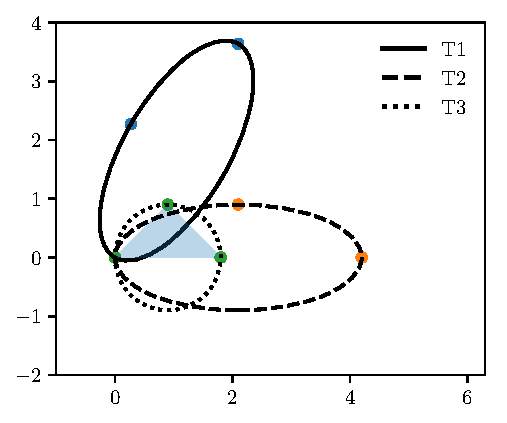
\includegraphics{tex/figures/scripts/circumscribed-circle}
	\fautor
	\label{fig:circumscribed-circle}
\end{figure}
\begin{equation}\label{eq:trpnts}
\varphi(p, \theta)=\left[\begin{array}{cc}
\frac{b}{a}&0\\
0&1
\end{array}\right]
\left[\begin{array}{cc}
\cos{\theta}&\sin{\theta}\\
-\sin{\theta}&\cos{\theta}
\end{array}\right]\left[\begin{array}{c}
p_x\\
p_y
\end{array}\right].
\end{equation}

Then, the problem to be solved is finding a circumscribed circle of the triangle formed by the points $(0, 0), \varphi(v, \theta)$ and $\varphi(w, \theta)$, such that the circle has radius $b$. As, for three non-colinear fixed points, there is always an unique circumscribed circle for the triangle formed by those three points, the only variable to be determined ends up being the angle of rotation $\theta$.

Let $A(\theta)$ be the area of the triangle formed by the points $(0, 0), \varphi(v, \theta)$ and $\varphi(w, \theta)$--note that the transformation does not preserve distance or area. Then, the radius $R$ of the circumscribed circle is given by \autoref{eq:circumscribed_circle} \cite[p.~189]{johnson1960}.

\begin{equation}\label{eq:circumscribed_circle}
R = \dfrac{\norm{\varphi(v, \theta)}\norm{\varphi(w, \theta)}\norm{\varphi(v, \theta)-\varphi(w, \theta)}   }{4A(\theta)}.
\end{equation}

Imposing the radius to be equal $b$ and squaring to eliminate the square roots present in the Euclidean distance, a function $\xi : [0, \pi) \mapsto \mathbb{R}_{>0}$ is defined by \autoref{eq:circumscribed_circle_b} in such a way that its zeros determine solutions to the E3PNT's instance. Two questions about $\xi(\theta)$ that arise are: is its set of roots finite? And, can they be found analytically?

\begin{equation}\label{eq:circumscribed_circle_b}
\xi(\theta) = 16b^2A(\theta)^2 - \norm{\varphi(v, \theta)}^2\norm{\varphi(w, \theta)}^2\norm{\varphi(v, \theta)-\varphi(w, \theta)}^2.
\end{equation}

According to \citeonline[p.~150]{powell}, any function of the form $\{\cos^j{x}\sin^k{x} : j, k \in \mathbb{N}\}$ can be written as a real trigonometric polynomial of degree $j+k$ which can have up to $2(j+k)$ different roots in the interval $[0, 2\pi)$. The reason to bring up this fact is that $\xi(\theta)$ can be written as $\sum_i^M c_i \cos^{j_i}(\theta)\sin^{k_i}(\theta)$, for some $M \in \mathbb{N}$ and $c_1, \dots, c_m \in \R$, which implies that it can have up to $2$ times its degree, denoted by $\max_{i\in \{1, \dots, M\}}$, zero.

 To show that, just note that it is possible to write $\norm{\varphi(v, \theta)}^2$ and $A(\theta)^2$ in that form, as it can be seen on \autoref{eq:dd} and \autoref{eq:dd2}, combine the parts as $\xi(\theta)$ is just addition and multiplication of terms in that form. It is also possible to see that the term of higher the degree of $\xi(\theta)$ is the multiplication of the three squared distances, as $\norm{\varphi(v, \theta)}^2$ has degree $2$ the degree of $\xi(\theta)$ is $6$.


\begin{align}\label{eq:dd}
	\norm{\varphi(v, \theta)}^2 = (v_x\frac{b}{a}\cos\theta + v_y\frac{b}{a}\sin\theta)^2 + (v_y\cos\theta - v_x\sin\theta)^2\\
	\label{eq:dd2} A(\theta)^2=\dfrac{1}{4}\det\left(
	\begin{array}{cc}
		v_x\frac{b}{a}\cos\theta + v_y\frac{b}{a}\sin\theta&v_y\cos\theta - v_x\sin\theta\\
		w_x\frac{b}{a}\cos\theta + w_y\frac{b}{a}\sin\theta&w_y\cos\theta - w_x\sin\theta
	\end{array}\right)^2
\end{align}

Because ellipses are symmetrical with respect to their major-axis, and any rotation in the interval $[0, \pi)$ is identical to a rotation in $[\pi, 2\pi)$, the number of different solutions is cut in half.
Therefore, the number of angles of rotation and centers that an ellipse of fixed shape can be placed, so it has three fixed points on its border is limited to $6$.

A possible approach to find all the roots of a high-degree polynomial is to find all the eigenvalues of its companion matrix\cite{horn}. There are methods that do that with the observation that roots not close to the origin are susceptible to large errors and some times can not be found. This was experienced in some instances where the method could not find any roots which were priorly known.
Therefore, Because there is no closed formula to find roots of polynomials of degree $12$ \cite{skopenkov2015}, and root-finding iterative methods, such as Newton's method, generally are not convergent for polynomials of degree $4$ or more \cite{mc1}, this approach is only useful to show the limitedness of the set of solutions. In the next section we present a method to approximate the roots of \autoref{eq:circumscribed_circle_b}.

\section{A method for E3PNT}

In this section we present a method for E3PNT and we try to make a case of it being correct, however, a proof is left as future work.

The idea of the method is to let two of the three points be fixed on the border of the ellipse and vary the angle to find it when the third point hits the border of the ellipse.

Let $u$ and $v$ be the pair out of the three points that are most distant from each other, also let $\theta_u \in [0, \pi)$ be the greatest $(E, u, v)$-feasible angle. Given an angle $\theta \in [0, \theta_u]$, let $q_\theta\in\R^2$ be a center of $E$, such that $\{u, v\} \subset \tilde{E}(q_\theta, \theta)$. Note that in general, there are two such centers, they could be told apart by their $y$-coordinate, and the method needs to be executed for both of them separately.
Then, a function $\rho : [0, \theta_u] \mapsto \R$ is defined to be the elliptical norm of the point $w$ with respect to $E(q_\theta, \theta)$.

\begin{equation}\label{eq:rho}
\rho(\theta) = \dfrac{\left((w-q_\theta)^T\left(\begin{array}{c}
	\cos{\theta}\\
	\sin{\theta}
	\end{array}\right)\right)^2}{a^2}+
\dfrac{\left((w-q_\theta)^T\left(\begin{array}{c}
	-\sin{\theta}\\
	\cos{\theta}
	\end{array}\right)\right)^2}{b^2}
\end{equation}

The angles such that \autoref{eq:rho} is equal to $1$ are the ones that are part of the solution and achieve three points on the border of the ellipse. From now on, a method is presented that tries to find those points in a efficient way. We conjecture that \autoref{eq:rho} is unimodal by parts, and we present a method that takes advantage of that.